\section{Compositional semantics and discourse processing}
% \subsection{Compositional semantics}
\begin{itemize}
	\item \textbf{Principle of Compositionality}: meaning of whole phrase derivable from meaning of its parts
	\item Sentence structure conveys some meaning as well
	\begin{itemize}
		\item Different syntactic structures may have the same meaning, but similar syntactic structures can also have different meanings
	\end{itemize}
	\item Not all phrases are interpreted compositionally (e.g. \textit{kick the bucket}) but can be grouped together and viewed as one element
	\item Meaning of a single word can depend on the composition (\textit{fast} programmer vs. \textit{fast} plane, metaphors,...)
\end{itemize}
\subsection{Compositional distributional semantics}
\begin{itemize}
	\item Extending distributional semantics to phrases/sentences
	\item Unsupervised model $\Rightarrow$ general-purpose representations
	\item Model composition in vector space. However, if we would model every sentence as independent, we would get an infinite dimensional space
\end{itemize}
\subsubsection{Vector mixture model}
\begin{itemize}
	\item Combining the vectors of all words in the sentence
	\item Mostly done either additive (adding all vector) or multiplicative (elementwise product of vectors)
	\item Problem: does not consider word order and is therefore suitable for modelling content words (nouns, verbs, adjectives,...), but not for function words that require syntactic dependencies (pronouns, ...)
	\item Is often used as baseline
\end{itemize}
\begin{figure}[ht]
	\centering
	\begin{subfigure}{0.3\textwidth}
		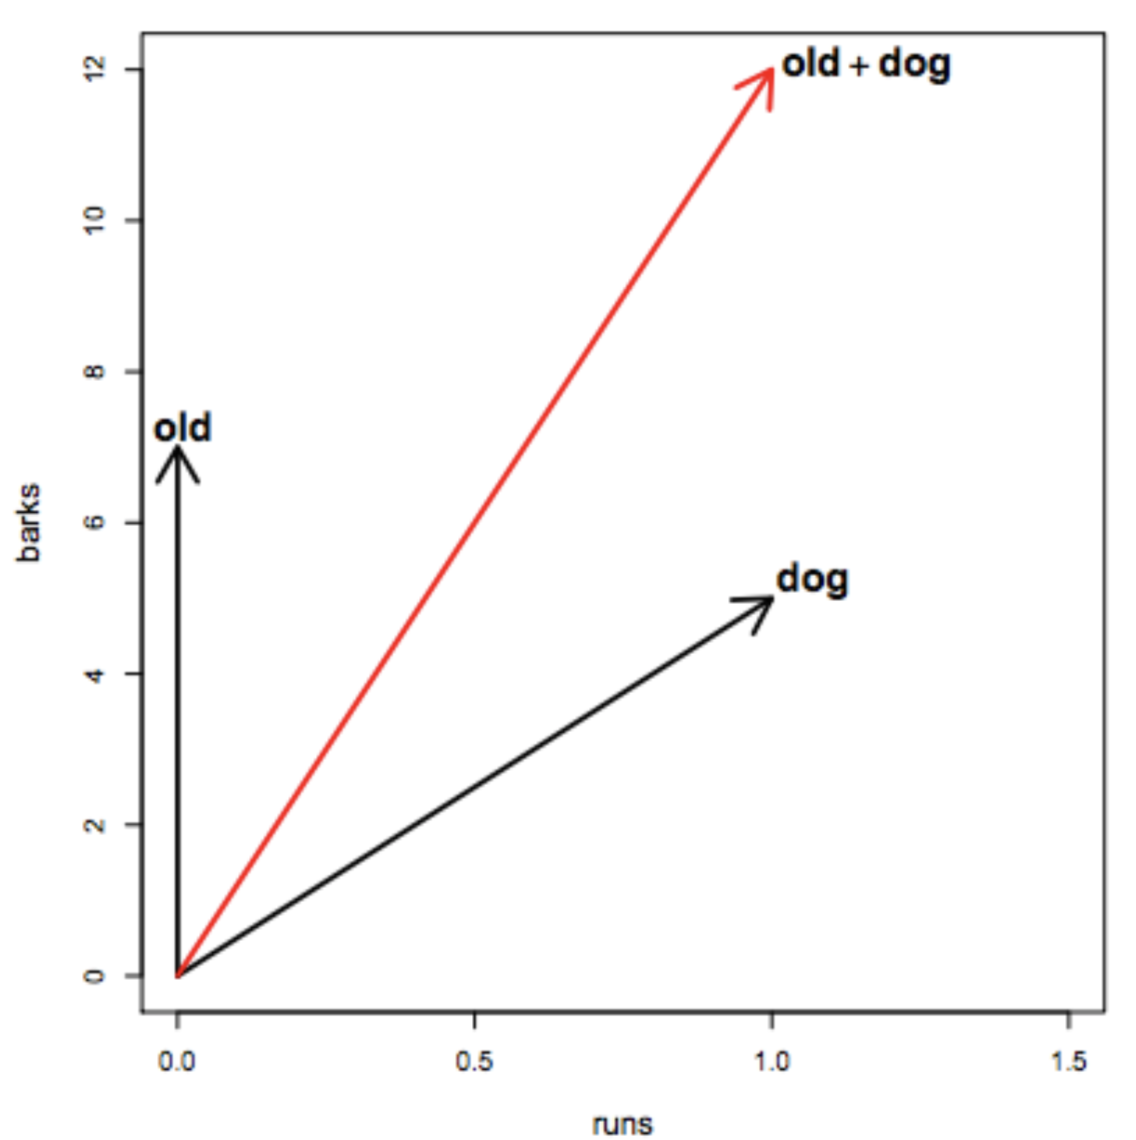
\includegraphics[width=\textwidth]{figures/compositional_semantic_vector_mixture_model.png}
		\caption{Vector mixture model}
	\end{subfigure}
	\begin{subfigure}{0.3\textwidth}
		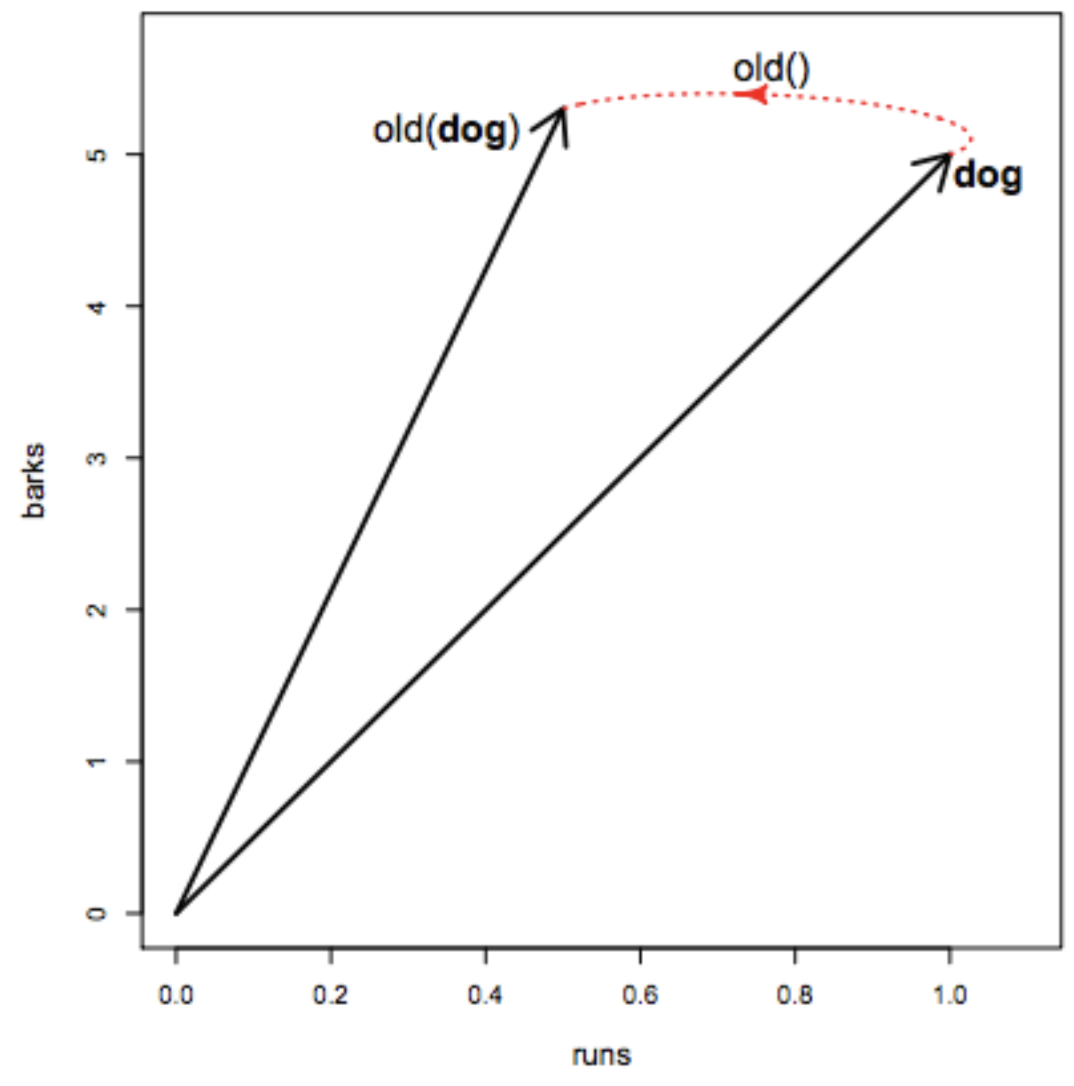
\includegraphics[width=\textwidth]{figures/compositional_semantics_lexical_function_models.png}
		\caption{Lexical function model}
	\end{subfigure}
	\caption{Compositional distributional semantics}
	\label{fig:compositional_semantic_vector_mixture_model}
\end{figure}
\subsubsection{Lexical function model}
\begin{itemize}
	\item Discriminate between words that meaning is determined by its context/distribution (e.g. nouns), and function words that are applied on the represented words as \textbf{lexical functions}
	\item Example: $\underbrace{\textit{old}}_{\text{functional}} \underbrace{\textit{dog}}_{\text{distributional}} \Rightarrow$ apply function of \textit{old} on \textit{dog}
	\item Lexical functions are parameter matrices (i.e. $\bm{A}_{\textit{old}}$) which are multiplied with the vector representation of nouns
	\begin{figure}[ht]
		\centering
		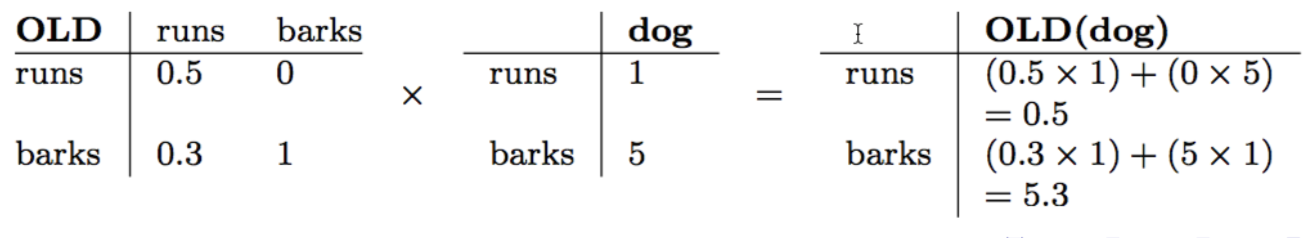
\includegraphics[width=0.5\textwidth]{figures/compositional_semantics_lexical_function_models_adjectives.png}
	\end{figure}
	\item Adjectives that does not change the meaning of a word are diagonal up to identity matrix $\Rightarrow$ element captures how features interact with each other given the adjective
	\item The matrices are learned by comparing the representation of plain nouns to combination of noun and adjective. Pseudo-code algorithm:
	\begin{enumerate}
		\item Obtain a distributional vector $n_j$ for each noun $n_j$ in the lexicon.
		\item Collect adjective noun pairs $(a_i,n_j)$ from the corpus.
		\item Obtain a distributional vector $p_{ij}$ of each pair $(a_i,n_j)$ from the same corpus using a conventional DSM.
		\item The set of tuples $\{(n_j,p_{ij})\}_j$ represents a dataset $\mathcal{D}(a_i)$ for the adjective $a_i$.
		\item Learn matrix $\bm{A}_i$ from $\mathcal{D}(a_i)$ using linear regression by minimizing:
		$$L(\bm{A}_i) = \sum\limits_{j\in \mathcal{D}(a_i)} ||p_{ij} - \bm{A}_i n_j||^2$$
	\end{enumerate} 
	\item Verbs can be represented as high-order tensors. If only subject is taken into consideration, it is a two-dimensional matrix. When also considering object, then it is three dimensional (or even higher)
	\item \textit{Polysemy} (different forms of a word) are mostly handled by a single representation. We assume that ambiguity can be handled as long as the context is given.
	\item To identify \textit{metaphors}, two separate senses of every adjective can be learned (literal and metaphorical). We then map from literal to metaphorical by a linear transformation. 
\end{itemize}
\subsubsection{Compositional semantics in neural networks}
\begin{itemize}
	\item Supervised learning framework $\Rightarrow$ compositional representations are fine-tuned for specific application/task
	\item Word representations are taken as input and processed within the network
	\item Example tasks include sentiment classification, paraphrasing, machine translation, ...
	\item Using recurrent and/or recursive networks (LSTMs, Tree-LSTMs, ...)
\end{itemize}
\subsection{Discourse structure}
\begin{itemize}
	\item Most documents have a implicit (in news paper articles, first sentence is a summary) or explicit structure like sections and paragraphs
	\item There are also relationships between sentences that need to be modeled as follow
\end{itemize}
\subsubsection{Rethorical relations}
\begin{itemize}
	\item There are implicit relations between sentences. For example:\\
	\texttt{Max fell. John pushed him.}\\
	can be interpreted as \textit{explanation} (Max fell because John pushed him), or as \textit{narration} (Max fell and then John pushed him).
	\item This relation is called \textbf{discourse relation} or \textbf{rhetorical relation}
	\item \textbf{Cue phrases} indicate what kind of relation it is. In the previous examples, the cue phrases were \texttt{because} and \texttt{and then}.
	\item Analyzing a text for rhetorical relations mostly gives a binary structure: the main sentence is called \textbf{nucleus}, and subsidiary phrase (explanation, justification, ...) is called \textbf{satellite}
	\item In a \textit{narration} (cue phrase \texttt{and}) both sentences have equal weight instead of nucleus vs satellite.
\end{itemize}
\subsubsection{Coherence}
\begin{itemize}
	\item Discourses need to have connectivity/context to be coherent.
	\item Otherwise, a sentence/small discourse might not make sense
	\item However, this information is mostly missing (background/world knowledge)!
	\item Assuming discourse coherence can affect interpretation. Especially when dealing with pronouns, th
\end{itemize}
\subsubsection{Overview of factors influencing discourse interpretation}
\begin{enumerate}
	\item \textit{Cue phrases} (\texttt{because}, \texttt{and}, ...)
	\item \textit{Punctuation and text structure} (\texttt{Max fell (John pushed him), and Kim laughed.})
	\item \textit{Real world context} (\texttt{Max was falling.} \texttt{John pushed him as he lay on the ground.})
	\item \textit{Tense and aspects} (\texttt{Max was falling.} \texttt{John pushed him.})
\end{enumerate}
\begin{itemize}
	\item Discourse parsing (understanding discourse structure) is a hard task
	\item Mostly done by supervision (annotated data of about 8-10 discourses)
	\item However, \textit{surface techniques} (primitive algorithms that look at characteristic phrases, punctuation, ...) seem to work to some extent
\end{itemize}
\subsection{Referring expressions and anaphora}
\begin{itemize}
	\item To fully process a discourse, co-references/referring expressions like pronouns need to be resolved
	\item We can define the following entities for a referring expression:
	\begin{itemize}
		\item \textit{referent} - a real world entity to which is referred
		\item \textit{referring expression} - part of speech that refers to an entity
		\item \textit{antecedent} - the text initially evoking a referent (where referent is named)
		\item \textit{anaphora} - the phenomenon of referring to an antecedent
		\item \textit{cataphora} - pronouns that appear \textit{before} the pronoun (rare)
	\end{itemize}
	\item \textbf{Pronoun resolution}
	\begin{itemize}
		\item Identifying the referents of pronouns
		\item \textit{Anaphora resolution}: in most cases, the task is limited to identifying referents that are mentioned before the actual pronoun/reference
	\end{itemize}
\end{itemize}
\subsubsection{Algorithms for anaphora resolution}
\begin{itemize}
	\item For anaphora resolution, we mostly apply a supervised training algorithm
	\item The instances in the corpus are possible pairs of pronoun and antecedent (possible antecedent include all noun phrases in the current and last 5 sentences)
	\item The classification is binary (true if pronoun refers to this specific antecedent, otherwise false)
	\item Training data is annotated by humans
	\item Beware that there are also pronouns in the text that might have no referent at all (\textit{pleonastic pronouns})
	\item Distinguishing between \textit{hard} and \textit{soft} constraints that must be fulfilled between pronouns and antecedent
	\item \textbf{Hard constraints} : Pronoun must match in terms of tense, singular/plural, gender, ...
	\item \textbf{Soft constraints/Salience}: 
	\begin{itemize}
		\item \textit{recency} -  more recent antecedents are preferred
		\item \textit{grammatical role} - subjects might be referred to more often than objects. Also, it is preferred that entity and pronoun has same role in sentence (subject, object, ...)
		\item \textit{repeated mention} - entities that have been mentioned more often are preferred
		\item \textit{coherence effect} - pronoun resolution might depend on discourse relation/semantic within the sentences
	\end{itemize}
	\item Based on the hard and soft constraints, we can define features for every pronoun-antecedent pair
	\item Simple classification model takes these features as input and classifies the link as valid or not
	\item Simplest evaluation matrix is link accuracy (number of correct links). However, it does not take into account pleonastic pronouns or a chain of references so that multiple metrics exist
\end{itemize}